\chapter{Model-Free Control}

La prima cosa che bisogna capire è la distinzione tra i seguenti due concetti:
\begin{compactitemize}
    \item \textbf{On-Policy Learning}: essenzialmente andiamo a utilizzare la stessa policy che andiamo ad aggiornare per muoverci all'intero dell'episodio: In termini tecnici si dice "Learn about policy $\pi$ from experience sampled from $\pi$.
    \item \textbf{Off-Policy Learning}: essenzialmente andiamo a utilizzare una policy (behavior) per muoverci all'interno degli episodi, e con quello che otteniamo andiamo ad aggioranre un'altra policy (target). In termini tecnici si dice "Learn about policy $\pi$ from experience sampled from $\mu$.
\end{compactitemize}

\subsection{Policy Iteration with Monte Carlo Evaluation}

Nel contesto del \textbf{model-free control}, l’obiettivo è determinare una policy ottimale senza assumere alcuna conoscenza esplicita del modello dell’MDP, ovvero senza conoscere né la funzione di transizione $P$ né la funzione di reward $R$. Questo vincolo ha conseguenze dirette sul modo in cui possono essere implementate le fasi di policy evaluation e policy improvement della policy iteration.

Si consideri innanzitutto il caso in cui si voglia applicare una classica relazione di policy iteration utilizzando la \textbf{state-value function} $v^\pi$. In un contesto model-based, il policy improvement si ottiene rendendo la policy greedy rispetto a $v^\pi$, cioè scegliendo, per ogni stato $s$, l’azione che massimizza l’espressione:
\[
R(s,a) + \gamma \sum_{s' \in \mathcal{S}} P(s' \mid s,a)\, v^\pi(s')
\]

Tuttavia, in un contesto model-free questa operazione non è realizzabile. Anche se fosse possibile stimare $v^\pi(s)$ tramite Monte Carlo, il passaggio di policy improvement richiede esplicitamente la conoscenza delle probabilità di transizione e dei reward attesi associati a ciascuna azione. In assenza del modello dell’MDP, non è possibile valutare l’effetto delle azioni sui futuri stati e, di conseguenza, non è possibile rendere la policy greedy rispetto alla state-value function.

Questo implica che una \textbf{policy iteration basata su $v^\pi$ non è compatibile con il paradigma model-free}. Il problema non risiede nella policy evaluation, che può essere effettuata tramite Monte Carlo usando l’esperienza episodica, bensì nel policy improvement, che richiede un one-step lookahead basato sul modello.

Per superare questa limitazione, il control model-free utilizza la \textbf{action-value function} $q^\pi(s,a)$. La funzione $q^\pi$ rappresenta il return atteso partendo dallo stato $s$, eseguendo l’azione $a$ e seguendo successivamente la policy $\pi$. A differenza di $v^\pi(s)$, essa associa direttamente un valore a ciascuna coppia stato–azione e incorpora implicitamente l’effetto della dinamica dell’ambiente.

Nel caso Monte Carlo, $q^\pi(s,a)$ può essere stimata come media dei ritorni osservati negli episodi ogni volta che la coppia $(s,a)$ viene visitata. Questo processo non richiede alcuna conoscenza del modello e si basa esclusivamente sull’esperienza campionata.

Una volta ottenuta una stima di $q^\pi$, il policy improvement diventa immediato: la policy viene aggiornata scegliendo, in ogni stato, l’azione che massimizza il valore dell’action-value function:
\[
\pi'(s) = \arg\max_{a \in \mathcal{A}} q^\pi(s,a)
\]
\begin{wrapfigure}{r}{0.4\textwidth}
    \centering
    \vspace{-10pt}
    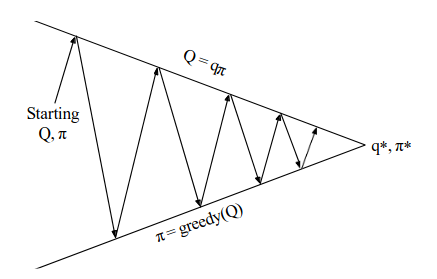
\includegraphics[width=\linewidth]{images/L51.png}
    \label{fig:TDlambda}
    \vspace{-10pt}
\end{wrapfigure}
Questo passo è completamente \textbf{model-free}, poiché non richiede né le probabilità di transizione né la funzione di reward. Tutta l’informazione necessaria per confrontare le azioni è contenuta nei valori stimati di $q^\pi$.

Il processo complessivo può quindi essere descritto come una \textbf{policy iteration model-free basata su action-value functions}, in cui:
\begin{compactitemize}
    \item la policy evaluation è realizzata tramite Monte Carlo estimation di $q^\pi$,
    \item la policy improvement è ottenuta rendendo la policy greedy rispetto a $q^\pi$.
\end{compactitemize}

Questo schema rientra nel quadro generale della \textbf{Generalized Policy Iteration}, in cui la stima di $q^\pi$ e l’aggiornamento della policy avvengono in modo iterativo fino alla convergenza verso l’action-value function ottimale $q^*$ e la policy ottimale $\pi^*$.

In sintesi, nel model-free control la scelta di lavorare con la action-value function non è solo conveniente, ma necessaria: mentre la state-value function non consente il policy improvement senza il modello dell’MDP, la action-value function permette di eseguire sia la valutazione sia il miglioramento della policy utilizzando esclusivamente l’esperienza osservata.
\begin{figure}[H]
    \centering
    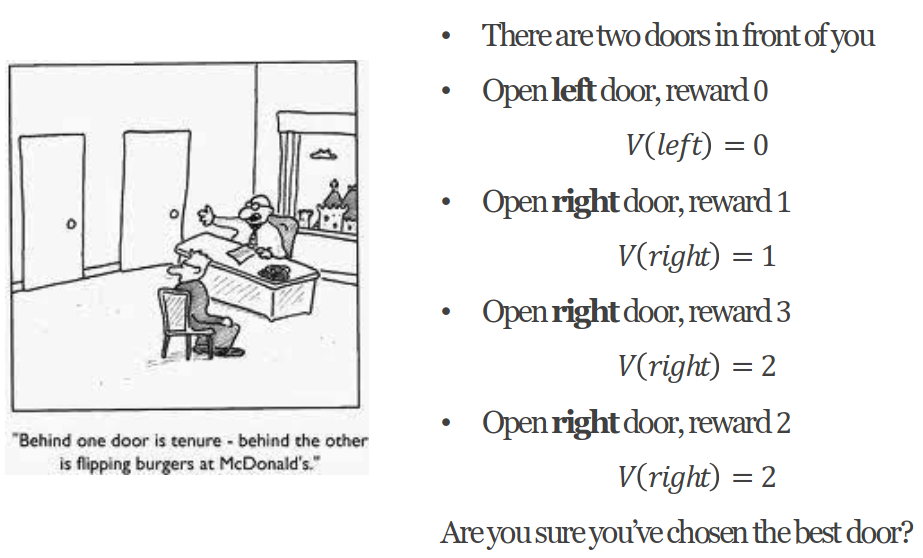
\includegraphics[width=0.7\textwidth]{images/L52.png}
    \caption{Esempio che mostra come, in presenza di reward stocastici o variabili nel tempo, una scelta apparentemente ottimale basata su poche osservazioni possa risultare subottimale. Sebbene una porta sembri inizialmente migliore, ulteriori esplorazioni possono rivelare valori medi diversi. L’esempio evidenzia quindi la necessità di bilanciare sfruttamento ed esplorazione, poiché basarsi solo sulla prima azione che massimizza il reward osservato non garantisce una decisione ottimale nel lungo periodo.}
    \label{fig:student_markov_chain}
\end{figure}

\section{$\epsilon$-Greedy Policies ed Exploration}

Nel control model-free, un problema centrale è garantire che l’agente continui a esplorare lo spazio delle azioni pur migliorando progressivamente la policy. Una policy puramente greedy, che seleziona sempre l’azione con valore stimato massimo, rischia infatti di convergere prematuramente verso una soluzione subottimale a causa di stime iniziali imprecise dei valori.

Una delle strategie più semplici ed efficaci per affrontare questo problema è l’uso delle \textbf{$\epsilon$-greedy policies}. L’idea fondamentale consiste nel bilanciare lo sfruttamento delle informazioni attualmente disponibili con una esplorazione casuale controllata.

Sia $Q(s,a)$ una stima dell’action-value function e sia $m = |\mathcal{A}|$ il numero di azioni disponibili. Una policy $\epsilon$-greedy rispetto a $Q$ è definita come:
\[
\pi(a \mid s) =
\begin{cases}
1 - \epsilon + \dfrac{\epsilon}{m} & \text{se } a \in \arg\max_{a' \in \mathcal{A}} Q(s,a') \\
\dfrac{\epsilon}{m} & \text{altrimenti}
\end{cases}
\]

Con probabilità $1 - \epsilon$ la policy seleziona un’azione greedy, ossia un’azione che massimizza il valore stimato $Q(s,a)$ nello stato $s$. Con probabilità $\epsilon$, invece, viene selezionata un’azione a caso, distribuita uniformemente tra tutte le azioni disponibili, incluse anche quelle greedy. In questo modo, tutte le azioni hanno sempre una probabilità strettamente positiva di essere esplorate.

Questa proprietà è cruciale nel model-free learning: garantire che ogni coppia stato–azione venga visitata sufficientemente spesso permette di migliorare progressivamente le stime di $Q(s,a)$ e ridurre l’effetto degli errori iniziali.


\subsection{$\epsilon$-Greedy Policy Improvement}

Le policy $\epsilon$-greedy non rappresentano soltanto una strategia di esplorazione, ma possono essere utilizzate anche come meccanismo di policy improvement all’interno della Generalized Policy Iteration.

Sia $\pi$ una policy $\epsilon$-greedy e sia $q^\pi$ la sua action-value function. Si consideri una nuova policy $\pi'$, definita come $\epsilon$-greedy rispetto a $q^\pi$. Per ogni stato $s$, il valore atteso di effettuare un’azione secondo $\pi'$ può essere scritto come:
\[
q^\pi\bigl(s, \pi'(s)\bigr)
= \sum_{a \in \mathcal{A}} \pi'(a \mid s)\, q^\pi(s,a)
\]

Sostituendo la definizione di policy $\epsilon$-greedy si ottiene:
\[
q^\pi\bigl(s, \pi'(s)\bigr)
=
\frac{\epsilon}{m} \sum_{a \in \mathcal{A}} q^\pi(s,a)
+
(1 - \epsilon) \max_{a \in \mathcal{A}} q^\pi(s,a)
\]

Poiché il valore massimo di $q^\pi(s,a)$ è sempre maggiore o uguale a qualunque combinazione convessa dei valori, segue che:
\[
\frac{\epsilon}{m} \sum_{a \in \mathcal{A}} q^\pi(s,a)
+
(1 - \epsilon) \max_{a \in \mathcal{A}} q^\pi(s,a)
\;\ge\;
\sum_{a \in \mathcal{A}} \pi(a \mid s)\, q^\pi(s,a)
=
v^\pi(s)
\]

Da questa disuguaglianza segue il seguente risultato fondamentale.

\medskip

\textbf{Teorema ($\epsilon$-Greedy Policy Improvement).}  
Per ogni policy $\epsilon$-greedy $\pi$, la policy $\pi'$ che è $\epsilon$-greedy rispetto a $q^\pi$ soddisfa:
\[
v^{\pi'}(s) \ge v^\pi(s) \qquad \forall s \in \mathcal{S}
\]

\medskip

Questo risultato mostra che il policy improvement non richiede necessariamente una policy puramente greedy. Anche introducendo esplorazione, è comunque garantito un miglioramento (o almeno un mantenimento) delle prestazioni in tutti gli stati.


\subsection{Monte Carlo Policy Iteration}
\begin{wrapfigure}{r}{0.4\textwidth}
    \centering
    \vspace{-10pt}
    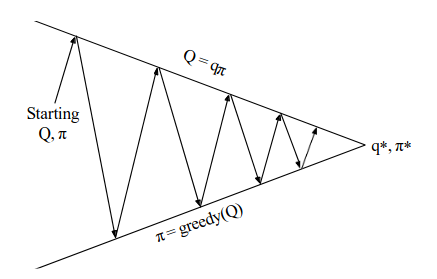
\includegraphics[width=\linewidth]{images/L51.png}
    \label{fig:TDlambda}
    \vspace{-10pt}
\end{wrapfigure}
Nel contesto del control model-free, la policy iteration può essere realizzata combinando:
\begin{compactitemize}
    \item una \textbf{policy evaluation} ottenuta tramite Monte Carlo estimation dell’action-value function,
    \item una \textbf{policy improvement} basata su una policy $\epsilon$-greedy.
\end{compactitemize}

Il processo parte da una stima iniziale di $Q$ e da una policy iniziale $\pi$. A ogni iterazione, vengono generati episodi completi seguendo la policy corrente $\pi$. Per ciascuna coppia stato–azione visitata, il valore $Q(s,a)$ viene aggiornato stimando il return medio osservato, ottenendo una nuova approssimazione di $q^\pi$.

Successivamente, la policy viene aggiornata rendendola $\epsilon$-greedy rispetto alla nuova stima di $Q$. Il procedimento può essere riassunto schematicamente come:
\[
Q \;\longrightarrow\; \pi = \epsilon\text{-greedy}(Q)
\;\longrightarrow\; Q \approx q^\pi
\;\longrightarrow\; \pi'
\]

Questo schema rappresenta una forma concreta di \textbf{Generalized Policy Iteration}, in cui policy evaluation e policy improvement avvengono in modo iterativo, approssimato e interdipendente. Al crescere del numero di episodi, e sotto opportune condizioni di esplorazione, il processo converge verso l’action-value function ottimale $q^*$ e una policy ottimale $\pi^*$.

\subsection{Monte Carlo Control}
\begin{wrapfigure}{r}{0.3\textwidth}
    \centering
    \vspace{-10pt}
    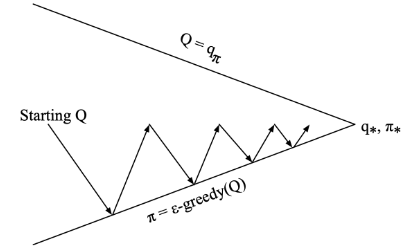
\includegraphics[width=\linewidth]{images/L53.png}
    \label{fig:TDlambda}
    \vspace{-10pt}
\end{wrapfigure}
Nel Monte Carlo Control, la policy evaluation e la policy improvement vengono eseguite dopo ogni episodio. Ogni episodio contribuisce a migliorare la stima di $Q$ e, di conseguenza, a rendere la policy sempre più orientata verso le azioni migliori, pur mantenendo una componente di esplorazione controllata tramite il parametro $\epsilon$.

In sintesi, l’uso di policy $\epsilon$-greedy consente di risolvere il problema del control in ambienti model-free garantendo contemporaneamente:
\begin{compactitemize}
    \item esplorazione continua di tutte le azioni,
    \item miglioramento monotono della policy,
    \item convergenza verso una policy ottimale.
\end{compactitemize}

\section{GLIE}

\subsection{Greedy in the Limit with Infinite Exploration}

Nel control model-free esiste una tensione fondamentale tra \textbf{esplorazione} e \textbf{sfruttamento}. Da un lato, per apprendere correttamente i valori delle azioni è necessario continuare a esplorare; dall’altro, per ottenere una policy ottimale nel lungo periodo è necessario agire in modo sempre più greedy rispetto alle stime dei valori.

Il concetto di \textbf{Greedy in the Limit with Infinite Exploration (GLIE)} formalizza una condizione che permette di risolvere questa tensione. Una sequenza di policy $\{\pi_k\}$ soddisfa la condizione GLIE se valgono entrambe le seguenti proprietà.

La prima proprietà è la \textbf{esplorazione infinita}. Ogni coppia stato–azione deve essere visitata un numero infinito di volte:
\[
\lim_{k \to \infty} N_k(s,a) = \infty \qquad \forall (s,a) \in \mathcal{S} \times \mathcal{A}
\]
Questa condizione garantisce che le stime dei valori non rimangano ancorate a osservazioni iniziali errate e che tutte le azioni abbiano la possibilità di essere valutate correttamente.

La seconda proprietà è la \textbf{convergenza greedily}. Nel limite, la policy deve diventare puramente greedy rispetto all’action-value function stimata:
\[
\lim_{k \to \infty} \pi_k(a \mid s)
=
\mathbf{1}\!\left(
a = \arg\max_{a' \in \mathcal{A}} Q_k(s,a')
\right)
\]
Nel lungo periodo, quindi, l’esplorazione viene progressivamente eliminata e la policy converge a una policy deterministica greedy.

Un esempio classico di policy GLIE è la policy $\epsilon$-greedy con un parametro di esplorazione decrescente nel tempo, ad esempio:
\[
\epsilon_k = \frac{1}{k}
\]
In questo caso, l’esplorazione è garantita per un tempo arbitrariamente lungo, ma tende a zero quando il numero di episodi cresce, assicurando una policy greedy nel limite.


\subsection{GLIE Monte-Carlo Control}

Il \textbf{GLIE Monte-Carlo Control} applica il principio GLIE all’algoritmo di Monte Carlo Control. L’idea è combinare:
\begin{compactitemize}
    \item una stima Monte Carlo dell’action-value function $q^\pi$,
    \item una policy $\epsilon$-greedy con $\epsilon$ decrescente nel tempo.
\end{compactitemize}

Il procedimento opera episodio per episodio. Al $k$-esimo episodio, viene generata una sequenza completa di stati, azioni e reward seguendo la policy corrente $\pi_k$:
\[
S_1, A_1, R_2, \dots, S_T \sim \pi_k
\]

Per ogni coppia $(S_t, A_t)$ visitata nell’episodio, viene incrementato il numero di visite:
\[
N(S_t, A_t) \leftarrow N(S_t, A_t) + 1
\]
e la stima dell’action-value function viene aggiornata tramite una media incrementale del return osservato:
\[
Q(S_t, A_t)
\leftarrow
Q(S_t, A_t)
+
\frac{1}{N(S_t, A_t)}
\Bigl(
G_t - Q(S_t, A_t)
\Bigr)
\]

Una volta aggiornati i valori $Q$, la policy viene migliorata rendendola $\epsilon_k$-greedy rispetto alla nuova stima:
\[
\pi_{k+1} = \epsilon_k\text{-greedy}(Q)
\]
con $\epsilon_k \to 0$ quando $k \to \infty$.

Questo schema soddisfa entrambe le condizioni GLIE: tutte le coppie stato–azione vengono esplorate infinitamente spesso e la policy diventa greedily ottimale nel limite. Di conseguenza, vale il seguente risultato fondamentale.

\medskip

\textbf{Teorema (Convergenza del GLIE Monte-Carlo Control).}  
Assumendo che l’MDP sia finito e che la sequenza di policy sia GLIE, l’algoritmo di GLIE Monte-Carlo Control converge con probabilità $1$ all’action-value function ottimale:
\[
Q(s,a) \longrightarrow q^*(s,a)
\qquad \forall (s,a) \in \mathcal{S} \times \mathcal{A}
\]
e la policy $\epsilon$-greedy converge a una policy ottimale $\pi^*$.

Questo risultato fornisce una garanzia teorica forte sulla correttezza del Monte Carlo Control, a patto di accettare l’ipotesi di episodi completi e una esplorazione sufficientemente lunga.


\subsection{Monte Carlo Control vs Temporal-Difference Control}

Sebbene il GLIE Monte-Carlo Control goda di solide garanzie teoriche, presenta alcune limitazioni pratiche. In particolare, l’aggiornamento dei valori avviene solo al termine di un episodio completo, una volta che il return totale $G_t$ è stato osservato. Questo rende il metodo intrinsecamente \textbf{offline} e comporta un’elevata varianza nelle stime.

Il \textbf{Temporal-Difference (TD) Control} nasce dall’idea di sostituire la stima Monte Carlo del return con una stima incrementale basata su informazioni parziali osservabili a ogni time-step. Invece di attendere la fine dell’episodio, il TD Control aggiorna direttamente l’action-value function dopo ogni transizione.

Dal punto di vista concettuale, il control TD mantiene la stessa struttura generale:
\begin{compactitemize}
    \item apprendimento diretto di $Q(s,a)$,
    \item policy improvement tramite policy $\epsilon$-greedy.
\end{compactitemize}

La differenza risiede nel metodo di valutazione. Mentre il Monte Carlo utilizza il return completo $G_t$, il TD Control utilizza una stima bootstrap che combina reward immediati e stime correnti dei valori futuri. Questo comporta diversi vantaggi: una varianza più bassa, la possibilità di apprendere online e la capacità di operare anche in presenza di sequenze incomplete o continue.

In questo senso, il TD Control può essere visto come un’evoluzione naturale del Monte Carlo Control, in cui la fase di policy evaluation viene resa più efficiente sostituendo il Monte Carlo con aggiornamenti temporally local. Questa idea costituisce la base di algoritmi fondamentali come SARSA e Q-learning, che rappresentano il fulcro del Reinforcement Learning model-free moderno.

\section{Sarsa Algorithm for On-Policy Control}

Il metodo \textbf{SARSA} è un algoritmo di control model-free e on-policy che apprende direttamente l’action-value function associata alla policy corrente. Il nome SARSA deriva dalla sequenza di variabili coinvolte nell’aggiornamento: stato $S_t$, azione $A_t$, reward $R_{t+1}$, stato successivo $S_{t+1}$ e azione successiva $A_{t+1}$.

Il controllo viene ottenuto applicando una \textbf{Generalized Policy Iteration} in cui policy evaluation e policy improvement avvengono a ogni time-step. L’algoritmo mantiene una stima $Q(s,a)$ dell’action-value function $q^\pi(s,a)$ e una policy $\pi$ tipicamente scelta come $\epsilon$-greedy rispetto a $Q$.

Ad ogni passo temporale, osservata la transizione $(S_t, A_t, R_{t+1}, S_{t+1}, A_{t+1})$, la stima di $Q$ viene aggiornata secondo la regola:
\[
Q(S_t, A_t) \leftarrow Q(S_t, A_t) + \alpha_t \, \delta_t
\]
dove il \textbf{TD-error} è definito come:
\[
\delta_t = R_{t+1} + \gamma Q(S_{t+1}, A_{t+1}) - Q(S_t, A_t)
\]

Questo aggiornamento è un esempio di \textbf{Temporal-Difference learning}, in cui il valore corrente viene corretto utilizzando una stima bootstrap del valore futuro invece di attendere il return completo. Poiché l’azione $A_{t+1}$ è selezionata dalla stessa policy che viene valutata, SARSA è un algoritmo intrinsecamente on-policy.

\begin{figure}[H]
    \centering
    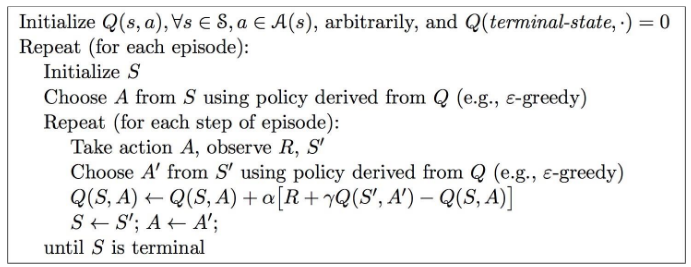
\includegraphics[width=0.9\textwidth]{images/L54.png}
    \caption{Algortimo Sarsa}
    \label{fig:student_markov_chain}
\end{figure}
\subsection{Convergence of Sarsa}

Sotto opportune condizioni, SARSA converge all’action-value function ottimale $q^*$ e la policy associata converge a una policy ottimale.

In particolare, la convergenza è garantita se la sequenza di policy $\{\pi_t\}$ soddisfa la condizione di \textbf{GLIE} e se i learning rates $\{\alpha_t\}$ soddisfano le condizioni di Robbins–Monro:
\[
\sum_{t=1}^{\infty} \alpha_t = \infty,
\qquad
\sum_{t=1}^{\infty} \alpha_t^2 < \infty
\]

La prima condizione assicura che ogni coppia stato–azione venga esplorata infinite volte, mentre la seconda garantisce che l’ampiezza degli aggiornamenti decresca sufficientemente nel tempo da stabilizzare le stime. Sotto queste ipotesi, la stima $Q(s,a)$ converge con probabilità $1$ alla funzione ottimale $q^*(s,a)$ e la policy $\epsilon$-greedy converge a una policy ottimale nel limite.


\subsection{n-Step Sarsa}

La versione standard di SARSA utilizza un aggiornamento a un singolo passo temporale (one-step), in cui il return è approssimato usando un solo reward futuro e la stima del valore al passo successivo. Questa idea può essere generalizzata introducendo i \textbf{n-step returns}, che combinano informazioni provenienti da più passi futuri.

Per $n = 1$, il one-step SARSA utilizza il return:
\[
q_t^{(1)} = R_{t+1} + \gamma Q(S_{t+1}, A_{t+1})
\]

Per $n = 2$, si ottiene:
\[
q_t^{(2)} = R_{t+1} + \gamma R_{t+2} + \gamma^2 Q(S_{t+2}, A_{t+2})
\]

Nel caso limite $n = \infty$, il return coincide con il return Monte Carlo:
\[
q_t^{(\infty)} = R_{t+1} + \gamma R_{t+2} + \gamma^2 R_{t+3} + \dots + \gamma^{T-1} R_T
\]

In generale, l’n-step Q-return è definito come:
\[
q_t^{(n)} =
R_{t+1}
+ \gamma R_{t+2}
+ \dots
+ \gamma^{n-1} R_{t+n}
+ \gamma^n Q(S_{t+n}, A_{t+n})
\]

L’aggiornamento di n-step SARSA diventa quindi:
\[
Q(S_t, A_t) \leftarrow Q(S_t, A_t)
+ \alpha \bigl( q_t^{(n)} - Q(S_t, A_t) \bigr)
\]

Variando il parametro $n$ è possibile ottenere un compromesso tra bias e varianza: valori piccoli di $n$ inducono maggiore bias ma minore varianza, mentre valori grandi di $n$ si avvicinano al comportamento Monte Carlo.


\subsection{Forward View Sarsa($\lambda$)}

L’algoritmo Sarsa($\lambda$) fornisce un meccanismo per combinare in modo continuo tutti gli n-step returns, senza dover scegliere esplicitamente un valore di $n$.

Nel \textbf{forward view}, si definisce il $\lambda$-return come una combinazione convessa di tutti gli n-step returns, pesata geometricamente:
\[
q_t^{\lambda}
=
(1 - \lambda)
\sum_{n=1}^{\infty}
\lambda^{n-1}
q_t^{(n)}
\]

Il parametro $\lambda \in [0,1]$ controlla l’importanza dei contributi a lungo termine. Per $\lambda = 0$ si ottiene il one-step SARSA, mentre per $\lambda \to 1$ il return tende al return Monte Carlo.

L’aggiornamento forward-view di Sarsa($\lambda$) è quindi:
\[
Q(S_t, A_t)
\leftarrow
Q(S_t, A_t)
+ \alpha \bigl( q_t^{\lambda} - Q(S_t, A_t) \bigr)
\]

Questa formulazione è principalmente di interesse teorico, poiché richiederebbe la conoscenza di ritorni futuri non ancora osservati.


\subsection{Backward View Sarsa($\lambda$)}

Per ottenere un algoritmo implementabile online, il forward view viene reso equivalente attraverso il \textbf{backward view}, che utilizza il concetto di \textbf{eligibility traces}. In questo approccio, viene mantenuta una traccia di eleggibilità per ogni coppia stato–azione.

Le eligibility traces sono inizializzate a zero:
\[
E_0(s,a) = 0 \qquad \forall (s,a)
\]

Ad ogni time-step, le tracce vengono aggiornate secondo:
\[
E_t(s,a) = \gamma \lambda E_{t-1}(s,a)
+ \mathbf{1}(S_t = s, A_t = a)
\]

In questo modo, le coppie stato–azione visitate recentemente mantengono un’eleggibilità elevata, che decade esponenzialmente nel tempo.

Il TD-error viene calcolato come nel SARSA standard:
\[
\delta_t = R_{t+1} + \gamma Q(S_{t+1}, A_{t+1}) - Q(S_t, A_t)
\]

Infine, l’action-value function viene aggiornata per tutte le coppie $(s,a)$ in proporzione al TD-error e alla rispettiva eligibility trace:
\[
Q(s,a) \leftarrow Q(s,a) + \alpha \, \delta_t \, E_t(s,a)
\]

Il backward view Sarsa($\lambda$) è computazionalmente efficiente, completamente online e, sotto opportune condizioni, equivalente al forward view in termini di comportamento asintotico.
\begin{figure}[H]
    \centering
    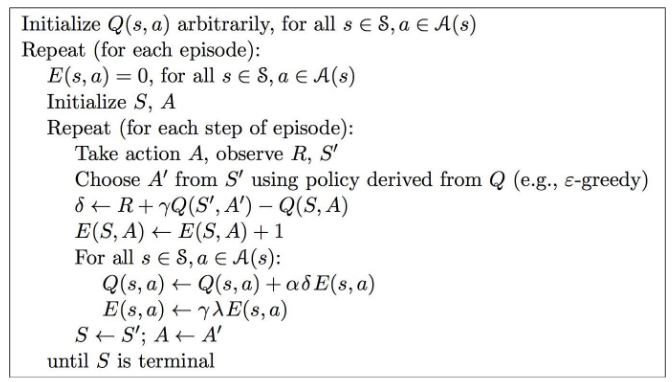
\includegraphics[width=0.9\textwidth]{images/L55.png}
    \caption{Algortimo Sarsa($\lambda$)}
    \label{fig:student_markov_chain}
\end{figure}

\section{Off-Policy Learning}

Nel Reinforcement Learning, il termine \emph{off-policy learning} indica la possibilità di valutare o migliorare una policy \emph{target} $\pi$ utilizzando esperienza generata da una policy diversa, detta \emph{behaviour policy} $\mu$. In questo contesto, l’obiettivo è stimare quantità come $v^\pi(s)$ o $q^\pi(s,a)$ mentre l’agente segue effettivamente la policy $\mu$.

Questa impostazione è particolarmente importante in diversi scenari pratici. Consente di apprendere osservando il comportamento di altri agenti o di esseri umani, di riutilizzare dati raccolti in passato con policy diverse e di apprendere una policy ottimale continuando a seguire una policy fortemente esplorativa. Inoltre, permette di valutare più policy differenti a partire da un’unica sorgente di esperienza.

Il problema centrale dell’off-policy learning è che le distribuzioni di probabilità indotte da $\pi$ e $\mu$ sugli episodi e sulle transizioni non coincidono. Per correggere questo disallineamento e ottenere stime corrette, è necessario introdurre il concetto di \textbf{importance sampling}.


\subsection{Importance Sampling}

L’importance sampling è una tecnica statistica che consente di stimare il valore atteso di una funzione rispetto a una distribuzione di probabilità utilizzando campioni generati da una distribuzione diversa.

Sia $X$ una variabile aleatoria e sia $f(X)$ una funzione integrabile. Il valore atteso di $f$ rispetto a una distribuzione $P$ è:
\[
\mathbb{E}_{X \sim P}[f(X)] = \sum_x P(x) f(x)
\]

Introducendo una seconda distribuzione $Q$, tale che $Q(x) > 0$ ogni volta che $P(x) > 0$, è possibile riscrivere l’aspettativa come:
\[
\mathbb{E}_{X \sim P}[f(X)]
=
\sum_x Q(x) \frac{P(x)}{Q(x)} f(x)
=
\mathbb{E}_{X \sim Q}
\left[
\frac{P(X)}{Q(X)} f(X)
\right]
\]

Il rapporto $\frac{P(X)}{Q(X)}$ è detto \textbf{importance sampling ratio} e misura quanto il campione estratto da $Q$ sia rappresentativo della distribuzione $P$. Applicando questa idea al Reinforcement Learning, l’importance sampling permette di correggere l’esperienza generata dalla behaviour policy $\mu$ affinché possa essere utilizzata per stimare quantità associate alla target policy $\pi$.

Una condizione fondamentale è che $\mu(a \mid s) > 0$ ogni volta che $\pi(a \mid s) > 0$; in caso contrario, il rapporto di importance sampling non è definito e l’apprendimento off-policy diventa impossibile.


\subsection{Importance Sampling for Off-Policy Monte-Carlo}

Nel contesto Monte-Carlo, l’obiettivo è stimare il return atteso sotto la policy target $\pi$ utilizzando episodi generati seguendo la behaviour policy $\mu$.

Poiché un episodio completo è una sequenza di azioni, è necessario correggere l’intero return utilizzando un prodotto di rapporti di importance sampling. Per un episodio che parte dal tempo $t$ e termina al tempo $T$, il coefficiente di correzione è definito come:
\[
\rho_{t:T}
=
\prod_{k=t}^{T}
\frac{\pi(A_k \mid S_k)}{\mu(A_k \mid S_k)}
\]

Il return corretto diventa quindi:
\[
G_t^{\pi/\mu} = \rho_{t:T} \, G_t
\]

La stima del valore viene aggiornata muovendosi verso questo return corretto:
\[
V(S_t)
\leftarrow
V(S_t) + \alpha
\bigl(
G_t^{\pi/\mu} - V(S_t)
\bigr)
\]

Questo aggiornamento è una stima non distorta di $v^\pi(s)$, ma presenta una criticità importante: poiché il coefficiente $\rho_{t:T}$ è un prodotto di molti termini, può crescere o decrescere molto rapidamente, causando un’elevata varianza nelle stime. In particolare, se $\pi$ e $\mu$ differiscono significativamente lungo l’episodio, il contributo di un singolo episodio può dominare l’intero apprendimento.

Per questo motivo, l’importance sampling Monte-Carlo è teoricamente corretto ma spesso poco stabile nella pratica.


\subsection{Importance Sampling for Off-Policy Temporal-Difference}

Nel caso dei metodi Temporal-Difference, l’off-policy learning può essere realizzato in modo più efficiente. A differenza del Monte-Carlo, gli aggiornamenti TD non dipendono dall’intero episodio, ma solo da una singola transizione.

Nel TD off-policy, il target viene corretto applicando l’importance sampling relativo a un solo passo temporale. L’aggiornamento assume la forma:
\[
V(S_t)
\leftarrow
V(S_t)
+
\alpha
\left(
\frac{\pi(A_t \mid S_t)}{\mu(A_t \mid S_t)}
\bigl(
R_{t+1} + \gamma V(S_{t+1})
\bigr)
-
V(S_t)
\right)
\]

In questo caso, il rapporto di importance sampling coinvolge soltanto la probabilità dell’azione effettivamente eseguita al tempo $t$. Non è necessario moltiplicare i rapporti lungo l’intero episodio, il che riduce drasticamente la varianza dell’aggiornamento.

Questa proprietà rende i metodi TD particolarmente adatti all’off-policy learning: le policy $\pi$ e $\mu$ devono essere sufficientemente compatibili solo localmente, su un singolo step, e non lungo l’intera traiettoria. Per questo motivo, i metodi off-policy basati su TD, come il Q-learning, risultano molto più stabili ed efficaci rispetto alle loro controparti Monte-Carlo basate su importance sampling.

\section{Q-Learning}

Il \textbf{Q-learning} è un algoritmo di control model-free e off-policy che apprende direttamente l’action-value function ottimale $q^*(s,a)$. A differenza di SARSA, il Q-learning separa esplicitamente la policy seguita dall’agente durante l’interazione con l’ambiente dalla policy utilizzata per la valutazione e il miglioramento, consentendo un apprendimento off-policy stabile ed efficiente.

L’obiettivo del Q-learning è stimare $q^*(s,a)$ senza assumere alcuna conoscenza del modello dell’MDP, utilizzando esclusivamente l’esperienza raccolta attraverso l’interazione con l’ambiente.


\subsection{Off-Policy Control with Q-Learning}

Nel Q-learning, l’agente seleziona le azioni seguendo una \textbf{behaviour policy} $\mu$, tipicamente scelta come $\epsilon$-greedy rispetto alla stima corrente di $Q(s,a)$. Questa policy garantisce un’adeguata esplorazione dello spazio delle azioni.

Tuttavia, l’aggiornamento dell’action-value function non dipende dall’azione effettivamente selezionata nel passo successivo, bensì dall’azione che massimizza il valore stimato nello stato successivo. In altre parole, la \textbf{target policy} $\pi$ è scelta come policy greedy rispetto a $Q$.

Formalmente, osservata la transizione $(S_t, A_t, R_{t+1}, S_{t+1})$, l’aggiornamento del Q-learning è definito come:
\[
Q(S_t, A_t)
\leftarrow
Q(S_t, A_t)
+
\alpha
\Bigl(
R_{t+1}
+
\gamma
\max_{a' \in \mathcal{A}}
Q(S_{t+1}, a')
-
Q(S_t, A_t)
\Bigr)
\]

Il termine di bootstrap utilizza il massimo sulle azioni possibili nello stato successivo, indipendentemente dall’azione scelta dalla behaviour policy. Questo consente di apprendere direttamente la policy ottimale continuando a seguire una policy esplorativa.

Una caratteristica cruciale del Q-learning è che questo aggiornamento non richiede alcuna correzione tramite importance sampling. Poiché il target è definito rispetto a un’azione massimizzante, e non rispetto all’azione effettivamente eseguita, l’algoritmo è intrinsecamente off-policy.


\subsection{Convergence of Q-Learning}

Il Q-learning gode di solide garanzie di convergenza. In particolare, se l’MDP è finito, se tutte le coppie stato–azione vengono visitate infinite volte e se i learning rates $\{\alpha_t\}$ soddisfano le condizioni di Robbins–Monro:
\[
\sum_{t=1}^{\infty} \alpha_t = \infty,
\qquad
\sum_{t=1}^{\infty} \alpha_t^2 < \infty,
\]
allora la stima $Q(s,a)$ converge con probabilità $1$ all’action-value function ottimale:
\[
Q(s,a) \longrightarrow q^*(s,a)
\qquad \forall (s,a) \in \mathcal{S} \times \mathcal{A}
\]

Di conseguenza, la policy greedy rispetto a $Q$ converge a una policy ottimale $\pi^*$.

È importante notare che, a differenza di SARSA, il Q-learning converge alla policy ottimale \emph{indipendentemente} dalla policy esplorativa utilizzata, purché questa garantisca un’esplorazione sufficiente. Questo rende il Q-learning particolarmente robusto e adatto a scenari in cui è necessario mantenere un’elevata esplorazione per lunghi periodi.


\subsection{Q-Learning Control Algorithm}

Il Q-learning può essere interpretato come una forma di Generalized Policy Iteration in cui policy evaluation e policy improvement sono completamente integrate in un singolo aggiornamento. A ogni time-step, il valore associato alla coppia $(S_t, A_t)$ viene spinto verso un target che include implicitamente il miglioramento greedy.

L’algoritmo può essere descritto come segue. A ogni passo temporale:
\begin{enumerate}
    \item dalla behaviour policy $\mu$ viene selezionata un’azione $A_t$ nello stato $S_t$;
    \item viene osservato il reward $R_{t+1}$ e lo stato successivo $S_{t+1}$;
    \item la stima di $Q(S_t, A_t)$ viene aggiornata tramite il target greedy.
\end{enumerate}

Formalmente, l’aggiornamento è:
\[
Q(S_t, A_t)
\leftarrow
Q(S_t, A_t)
+
\alpha
\Bigl(
R_{t+1}
+
\gamma
\max_{a' \in \mathcal{A}} Q(S_{t+1}, a')
-
Q(S_t, A_t)
\Bigr)
\]

Nel lungo periodo, questo schema consente di apprendere simultaneamente la value function ottimale e la policy ottimale, costituendo uno dei pilastri fondamentali del Reinforcement Learning model-free.
\begin{figure}[H]
    \centering
    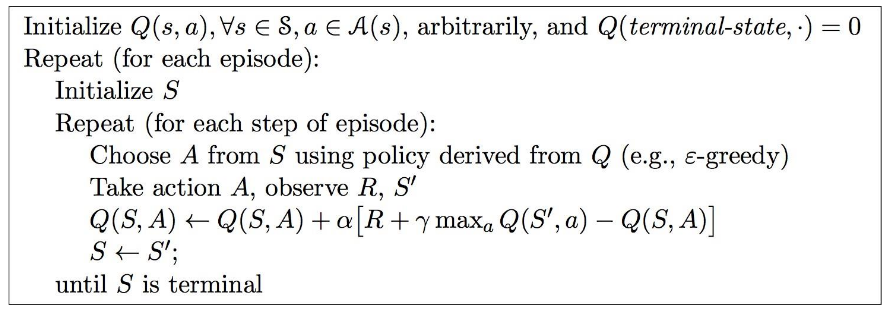
\includegraphics[width=0.7\textwidth]{images/L56.png}
    \caption{Algortimo Q-Learning}
    \label{fig:student_markov_chain}
\end{figure}

\begin{figure}[H]
    \centering
    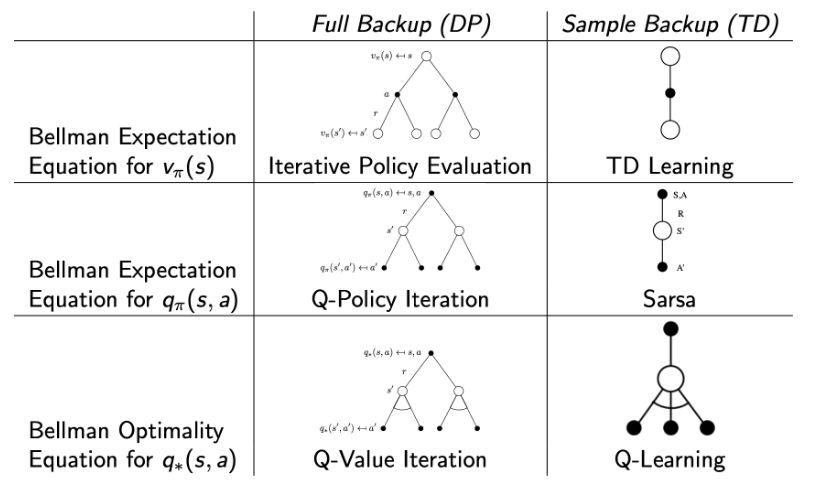
\includegraphics[width=0.7\textwidth]{images/L57.png}
    \caption{Relationship between DP and TD}
    \label{fig:student_markov_chain}
\end{figure}

\begin{figure}[H]
    \centering
    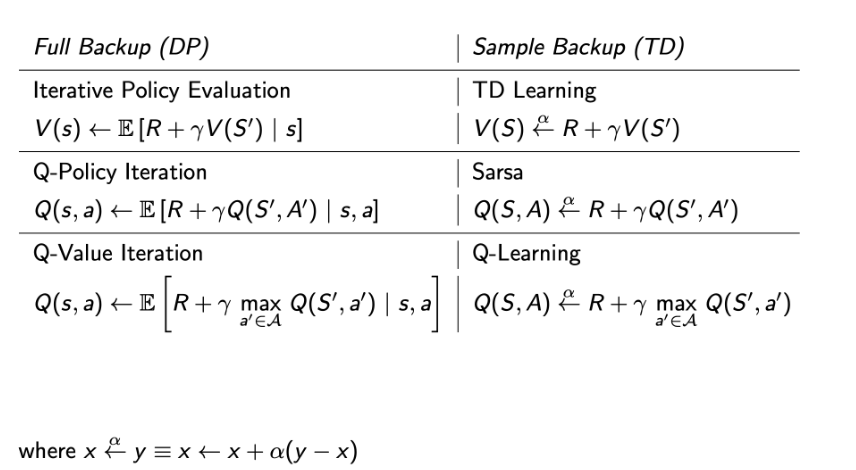
\includegraphics[width=0.7\textwidth]{images/L58.png}
    \caption{Relationship between DP and TD}
    \label{fig:student_markov_chain}
\end{figure}
